% !TeX program = lualatex
% Draft workspace for the JSCE paper associated with the SLSC project.
% Open this file in VS Code and build with latexmk + lualatex.
\documentclass{jjsce}
% \documentclass[jscefinal]{jjsce}

\usepackage{amsmath}
\usepackage{amsthm}
\usepackage{iftex}
\usepackage[defaultsups]{newtxtext}
\usepackage[varg]{newtxmath}
\usepackage{bm}
\usepackage{siunitx}
\usepackage[superscript]{cite}
\usepackage{url}
\usepackage{endnotes}
\usepackage[savepos]{zref}
\ifLuaTeX
\usepackage{graphicx}
\usepackage[luatex,pdfencoding=auto]{hyperref}
\else
\usepackage[dvipdfmx]{graphicx}
\usepackage[dvipdfmx]{hyperref}
\usepackage{pxjahyper}
\fi
\usepackage{jjsce-macros}

\aboveEtitlesep20mm
\setlength{\textfloatsep}{1.0\Cvs plus 2pt minus 2pt}
\setlength{\dbltextfloatsep}{1.0\Cvs plus 2pt minus 2pt}

\newcommand{\SLSC}{\mathrm{SLSC}}
\newcommand{\AIC}{\mathrm{AIC}}

% 共著者確認用の修正表示. 投稿時は revisioncolor を black にする.
\newcommand{\revisioncolor}{black}
% \renewcommand{\revisioncolor}{black}
\newcommand{\rev}[1]{\textcolor{\revisioncolor}{#1}}

% 共著者確認用の付録を出力する場合は true, 投稿時に外す場合は false にする.
\newif\ifshowappendix
% \showappendixtrue
\showappendixfalse
\AtEndDocument{%
  \ifshowappendix
    \clearpage
    \onecolumn
    \appendix
    % This appendix is for coauthor checking. Toggle it in main.tex.
\section{計算で用いた分布とパラメータ}
\label{app:distribution_defs}

本付録では, 数値計算で用いた分布のパラメータ化, 確率密度関数, および主要な計算条件をまとめる. 
ここで, \(\Gamma(\cdot)\) はガンマ関数を表す.

\subsection{確率密度関数}

\noindent\textbf{Gumbel 分布.}
\(\alpha\) を位置母数, \(\beta>0\) を尺度母数とし, \(z=(x-\alpha)/\beta\) とおく. 
このとき
\[
f(x;\alpha,\beta)
=
\frac{1}{\beta}
\exp\{-z-\exp(-z)\},
\quad -\infty<x<\infty .
\]

\noindent\textbf{一般化極値分布 (GEV).}
\(\mu\) を位置母数, \(\sigma>0\) を尺度母数, \(k\) を形状母数とし,
\[
t=1+k\frac{x-\mu}{\sigma}
\]
とおく. 
\(t>0\) の範囲で, \(k\ne0\) のとき
\[
f(x;k,\sigma,\mu)
=
\frac{1}{\sigma}
t^{-1/k-1}
\exp\{-t^{-1/k}\}
\]
である. 
\(k=0\) は Gumbel 分布への極限として扱った.

\noindent\textbf{対数ピアソンIII型分布 (LP3).}
\[
\log X = c + aY,\quad Y\sim \mathrm{Gamma}(b,1)
\]
とし, \(a>0\), \(b>0\) とする. 
\(z=(\log x-c)/a\) とおくと, \(x>\exp(c)\) に対して
\[
f(x;a,b,c)
=
\frac{z^{b-1}\exp(-z)}
{a x \Gamma(b)}
\]
である.

\noindent\textbf{平方根指数型最大値分布 (SqrtEt).}
\(a>0\), \(b>0\) とする. 
\(x\ge0\) に対して
\[
f(x;a,b)
=
\frac{ab}{2}
\exp\left[
-\sqrt{bx}
-a\left(1+\sqrt{bx}\right)\exp\{-\sqrt{bx}\}
\right]
\]
である.

\noindent\textbf{平行移動指数分布 (Exp).}
\(c\) を位置母数, \(\mu>0\) を尺度母数とする. 
\(x\ge c\) に対して
\[
f(x;c,\mu)
=
\frac{1}{\mu}
\exp\left\{-\frac{x-c}{\mu}\right\}
\]
であり, \(x<c\) では \(f(x)=0\) とする.

\noindent\textbf{3母数対数正規分布 (LN3).}
\(c\) を位置母数, \(\mu_L\) と \(\sigma_L>0\) を対数空間での位置母数および尺度母数とする. 
\[
y=\frac{\log(x-c)-\mu_L}{\sigma_L}
\]
とおくと, \(x>c\) に対して
\[
f(x;c,\mu_L,\sigma_L)
=
\frac{1}{(x-c)\sigma_L\sqrt{2\pi}}
\exp\left(-\frac{y^2}{2}\right)
\]
である.

\subsection{真の分布として用いたパラメータ}

\begin{center}
\small
\setlength{\tabcolsep}{5pt}
\begin{tabular}{lll}
\hline
分布 & パラメータ & 値 \\
\hline
Gumbel & \(\alpha,\beta\) & \(97.7438,\ 30.7042\) \\
GEV & \(k,\sigma,\mu\) & \(0.0910,\ 29.5452,\ 96.2345\) \\
LP3 & \(a,b,c\) & \(0.0683,\ 24.3314,\ 3.0352\) \\
SqrtEt & \(a,b\) & \(190.2683,\ 0.5685\) \\
Exp & \(c,\mu\) & \(54.5000,\ 61.6320\) \\
LN3 & \(c,\mu_L,\sigma_L\) & \(31.3965,\ 4.3254,\ 0.4805\) \\
\hline
\end{tabular}
\end{center}

\subsection{主な計算条件}

\begin{center}
\small
\setlength{\tabcolsep}{5pt}
\begin{tabular}{ll}
\hline
項目 & 設定 \\
\hline
標本サイズ & \(N=50,100,150\) \\
反復数 & \(100\) \\
乱数シード & \(42\) \\
プロッティングポジション & Cunnane 式 \\
SLSC 閾値 & \(0.04\) \\
ジャックナイフ幅の参照再現期間 & \(T_{\mathrm{ref}}=100\) \\
\hline
\end{tabular}
\end{center}

  \fi
}

\begin{document}

\jtitle{SLSC に基づく水文頻度解析の\\適合度評価に関する統計的再検討}
\etitle{A STATISTICAL REASSESSMENT OF GOODNESS-OF-FIT EVALUATION IN HYDROLOGICAL FREQUENCY ANALYSIS BASED ON SLSC}

\authorlist{%
 \authorentry{小柴 孝太}{Takahiro KOSHIBA}{TK}
 \authorentry{田中 智大}{Tomohiro TANAKA}{TT}
 \authorentry{平賀 優介}{Yusuke HIRAGA}{YH}
 \authorentry{清水 啓太}{Keita SHIMIZU}{KS}
 \authorentry{丸谷 靖幸}{Yasuyuki MARUYA}{YM}
 \authorentry{風間 聡}{So KAZAMA}{SK}
 \authorentry{北野 利一}{Toshikazu KITANO}{TK2}
	}
\Jbreakauthorline{4}
\breakauthorline{4}
\Caffiliate[TK]{正会員　博（工）京都大学防災研究所 助教（\jipcode{612--8235}京都府京都市伏見区横大路下三栖東ノ口）}{koshiba.takahiro.4s@kyoto-u.ac.jp}
\Caffiliate[TT]{正会員　博（工）京都大学防災研究所 准教授（\jipcode{611--0011}京都府宇治市五ケ庄）}{}
\Caffiliate[YH]{正会員　Ph.D. 東北大学大学院工学研究科 助教（\jipcode{980--8579}宮城県仙台市青葉区荒巻字青葉6-6-06）}{}
\Caffiliate[KS]{正会員　博（工）北海道大学大学院工学研究院 特任助教（\jipcode{060--8628}北海道札幌市北区北十三条西8）}{}
\Caffiliate[YM]{正会員　博（工）九州大学大学院工学研究院 准教授（\jipcode{819--0395}福岡県福岡市西区元岡744）}{}
\Caffiliate[SK]{正会員　博（工）東北大学大学院工学研究科 教授（\jipcode{980--8579}宮城県仙台市青葉区荒巻字青葉6-6-06）}{}
\Caffiliate[TK2]{正会員 博（工）名古屋工業大学大学院工学研究科 教授（\jipcode{466--8555}愛知県名古屋市昭和区御器所町）}{}
% \received{2026}{4}{5}
% \accepted{2026}{4}{5}

\begin{abstract}
本稿は, 水文頻度解析で用いられる標準最小二乗規準 (SLSC) について, 標本サイズ依存性と標準化の影響を再検討した.
6分布を対象としたモンテカルロ計算により, SLSC は標本サイズの増加とともに低下する傾向を示した.
また, \(X\) 空間と \(S\) 空間を区別し, 非線形標準化では SLSC が標準化関数に依存する距離評価となることを示した.
特に LN3 の \(S\) 空間評価は小さい値を与えやすく, 分布間比較に影響しうる.
\rev{さらに, SLSC+ジャックナイフ法と AIC の採択結果も比較した.}
SLSC の解釈には, 固定閾値だけでなく, 標準変量の定義と距離尺度の違いを明示する必要がある.

\end{abstract}

\begin{Eabstract}
This study reexamines the Standard Least-Squares Criterion (SLSC) used in hydrological frequency analysis, focusing on sample-size dependence and the effect of standardization. Monte Carlo simulations for six distributions show that SLSC tends to decrease as sample size increases. By distinguishing the original data space (X-space) from the standardized plotting-paper space (S-space), the analysis shows that nonlinear standardization makes SLSC a distance measure that depends on the standardizing function. In particular, the S-space evaluation of LN3 tends to give small SLSC values and can affect comparisons among distributions. The outcomes of the SLSC+jackknife procedure and AIC were also compared. These results indicate that SLSC should be interpreted with attention to fixed thresholds, the definition of the standard variate, and the resulting distance scale.

\end{Eabstract}

\begin{keyword}
hydrological frequency analysis, SLSC, AIC, goodness-of-fit, Monte Carlo simulation
\end{keyword}

\maketitle

\section{はじめに}
水文頻度解析における確率分布の選択は, 設計外力の推定値に直接影響する重要な手続きである.
日本では, 水文頻度解析の考え方, 用いられる確率分布, 母数推定法および適合度評価法について, 早くから体系的な整理が行われてきた{\cite{Takara1998}}.
とくに, 宝・高棹は, 確率分布モデルの適合度と確率水文量の変動性を併せて評価する枠組みを提示し, 標準最小二乗規準（以下, SLSC）を実務的な適合度評価指標として位置づけた{\cite{TakaraTakasao1988}}.
\rev{SLSC は, 確率紙上の視覚的一致性を数量化しようとする指標であり, 確率紙上の直線性を相関係数で評価する Filliben の正規性検定や, Kinnison による Gumbel 分布の相関係数適合度検定とも同系統の発想に立つものとみなせる{\cite{Filliben1975,Kinnison1989}}.}

その一方で, SLSC の統計的意味や運用の妥当性については, 既にいくつかの問題点が指摘されている.
葛葉は, SLSC 自体が確率変数であり, 固定値による判定ではなく, 標本サイズに応じて閾値を考えるべきことを論じた{\cite{Kuzuha2010}}.
藤部は, モンテカルロ計算により, SLSC が標本サイズに依存して小さくなること, 固定閾値 $0.04$ による判定が安定的でないことを示した.
また, 再現期待値のバイアスと推定幅の比較から, 3母数分布間の選択による実用上の改善が限定的であることを指摘した{\cite{Fujibe2011}}.
林らは, SLSC を検定統計量として扱う試みを示したが, SLSC の分布が標本サイズや想定分布に依存し, 3母数型モデルに対して一般的な取扱いが困難であることを報告している{\cite{HayashiEtAl2012}}.
また, 葛葉・水木は, 従来の手引きに基づく手続きにおいて, SLSC が標本サイズおよび確率分布に関して一律には比較しにくいことを整理し, その修正法や適用上の留意点を提案している{\cite{KuzuhaMizuki2021,KuzuhaMizuki2022}}.

以上の既往研究により, SLSC の固定閾値運用や標本サイズ依存性の問題はかなり明らかになってきた.
しかし, SLSC の計算において, 観測値と理論値をいかなる空間で比較しているのか, すなわち標準化の役割そのものを整理した議論は十分ではない.
線形標準化であれば, それは位置と尺度の調整に過ぎず, 観測値の空間における距離評価と本質的に同値である.
これに対し, 対数変換を含む標準化のように非線形標準化を用いる場合には, SLSC の値は標準化関数に依存した距離評価となり, 分布間で同一の距離尺度を共有しているとは限らない.
しかし, 実務上は, 標準変量の定義の違いが SLSC の比較可能性に与える影響は必ずしも明示されてこなかった.
また, 実務における分布選択は, 単純な最小 SLSC ではなく, 一定の閾値を満たす候補の中からジャックナイフ法により推定幅の小さい分布を選ぶ手順として運用されることが多い{\cite{Fujibe2011}}.
したがって, 現在の実務に即した形で SLSC 系規準の位置づけを再検討するには, SLSC の値そのものの挙動に加え, SLSC+ジャックナイフ法および情報量規準による採択結果との比較が必要である.

そこで本稿では, SLSC の比較空間を二つに分けて考える.
すなわち, 観測値と理論分位を実データの空間で比較する立場を, 本稿では便宜的に X 空間, 標準化後の確率紙上の空間で比較する立場を S 空間と呼ぶ.
本稿の関心は, これらを明確に区別した上で, とくに S 空間における非線形標準化が適合度評価にどのような偏りを導くかを理論と数値計算の両面から再検討することにある.

本稿では, グンベル分布 (Gumbel), 一般化極値分布 (GEV), 対数ピアソンIII型分布 (LP3), 平方根指数型最大値分布 (SqrtEt), 平行移動指数分布 (Exp), 3母数対数正規分布 (LN3) の6分布を対象として, 多数回のモンテカルロ計算を実施した.
\rev{これらの分布は, 日本の実務で用いられてきた水文統計ユーティリティー Ver. 1.5 で扱われる分布を踏まえて選定した{\cite{JICE2003}}.}
本稿の目的は, 既往研究で指摘されてきた問題を踏まえつつ, 次の三点を明確にすることである.
第一に, SLSC の標本サイズ依存性が6分布比較に拡張しても維持されるかを確認する.
第二に, SLSC の値が線形変換では不変である一方, 非線形標準化では標準化関数に依存した距離評価となることを示す.
第三に, SLSC+ジャックナイフ法と AIC による採択結果を比較し, 実際の分布選択手順における SLSC 系規準の位置づけを再確認する.

以下, 2章で方法, 3章で結果, 4章で考察, 5章で結論を示す.


\section{方法}
本稿では, SLSC の性質を確認するために, 真の分布から独立同分布標本を生成し, 各候補分布を当てはめた上で適合度指標を比較するモンテカルロ計算を行った.
対象分布は, Gumbel, GEV, LP3, SqrtEt, Exp, LN3 の6分布である.
各分布について, 真の分布として標本を発生させる場合と, 当てはめ分布として用いる場合の両方を考えた.

\subsection{SLSC の定義}
日本の水文頻度解析で一般に用いられてきた SLSC は, 観測値 $x_{(i)}$ を標準変量 $s=f(x)$ に写像した空間で, 観測値と理論値のずれを評価する指標である.
観測値の順序統計量に対応する標準変量を $s_{(i)}$, モデル分布に基づく理論値を $s_{(i)}^{\ast}$ とすると, SLSC は
\begin{equation}
\mathrm{SLSC}
=
\frac{
\sqrt{\dfrac{1}{N}\sum_{i=1}^{N}\bigl(s_{(i)}-s_{(i)}^{\ast}\bigr)^2}
}{
\left|s_q^{\ast}-s_{1-q}^{\ast}\right|}
\label{eq:slscs}
\end{equation}
と定義される. ここで, $q$ は上側分位を表す定数であり, 実務では $q=0.99$ が多く用いられる.
本稿では便宜的に, これを \(S\) 空間における SLSC と呼ぶ.

これに対し, 実データの空間で直接
\begin{equation}
\mathrm{SLSC}_x
=
\frac{
\sqrt{\dfrac{1}{N}\sum_{i=1}^{N}\bigl(x_{(i)}-x_{(i)}^{\ast}\bigr)^2}
}{
\left|x_q^{\ast}-x_{1-q}^{\ast}\right|}
\label{eq:slscx}
\end{equation}
と定義される量も考える.
同様に, これを \(X\) 空間における SLSC と呼ぶ.
葛葉・水木\cite{KuzuhaMizuki2022} でも指摘されているように, 標準変量が線形変換である場合には, \eqref{eq:slscs} と \eqref{eq:slscx} は一致する.
他方, 標準変量が非線形である場合には, \eqref{eq:slscs} と \eqref{eq:slscx} は一般に一致しない.
そこで本稿では, 以後 \(S\) 空間と \(X\) 空間を明示的に区別して記述し, 両者の理論的な関係は次節で整理する.

標準変量の定義は一般に一意ではなく, 代表的な定義は EVA の技術資料にも整理されている{\cite{DHI2022}}.
\rev{本稿では, \tabref{tab:standard_variate}の標準変量 $s=f(x)$ を比較用の簡易定義として用いた（GEV, LP3, SqrtEt などには形状母数を含む別定義もあり得る）.}
表の定義では, LP3 と LN3 の標準変量はいずれも元の \(x\) に対して非線形であり, それらの \(S\) 空間 SLSC は \(X\) 空間 SLSC と同一ではない.
本稿では, 非線形標準化の影響を具体的に示す代表例として, LN3 について表に示した対数標準化による \(S\) 空間評価に加えて, \(X\) 空間評価も行った.

\begin{table}[tb]
\caption{本研究で用いた標準変量 $s=f(x)$}
\label{tab:standard_variate}
\centering
\small
\setlength{\tabcolsep}{4pt}
\begin{tabular}{ll}
\hline
分布 & 標準変量 $f(x)$ \\
\hline
Gumbel & $(x-\alpha)/\beta$ \\
GEV    & $(x-\mu)/\sigma$ \\
LP3    & $\{\log x-c\}/a$ \\
SqrtEt & $bx$ \\
Exp    & $(x-c)/\mu$ \\
LN3    & $\{\log(x-c)-\mu_L\}/\sigma_L$ \\
\hline
\end{tabular}
\end{table}

\subsection{X 空間と S 空間の関係}
前節では, SLSC を \(S\) 空間と \(X\) 空間の二通りに定義した.
ここでは, 両者がどのような条件で一致し, どのような場合に異なる規準となるかを整理する.

確率紙を主たる道具としていた時代には, 確率紙上にデータをプロットし, 理論直線からのずれをその空間で評価するという発想自体は自然であった.
\figref{fig:probpaper_to_linear} は, その点を模式的に示したものである.
\figref{fig:probpaper_to_linear}(a)のように, 確率紙に相当する座標では理論関係は直線として表されるため, 標本点と理論直線の距離を測ることには手続き的な納得性がある.
しかし, 同じ関係を\figref{fig:probpaper_to_linear}(b)のように元の線形軸へ戻すと, 理論関係は一般には曲線となり, 確率紙上で同程度に見えるずれが, 元の雨量空間では異なる大きさの差に対応する.
さらに, \figref{fig:probpaper_to_linear}(c)は, この差が位置に依存する重みとして現れることを示している.
したがって, 非線形標準化を介した \(S\) 空間の SLSC は, 元の \(X\) 空間での単純な二乗平均平方根誤差ではなく, 位置依存の重みを伴う量として理解されるべきである.

\begin{figure}[tb]
  \centering
  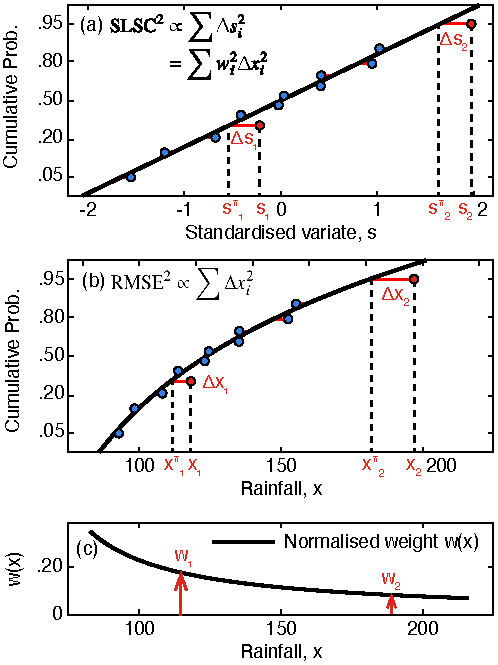
\includegraphics[width=\linewidth]{fig/method/probpaper_linear_weights_ln3_3panel_edited.pdf}
  \caption{非線形標準化における誤差評価の模式図.
  (a) 確率紙に相当する \(S\) 空間では理論関係は直線となる.
  (b) 同じ関係を雨量の \(X\) 空間へ戻すと曲線となる.
  (c) 非線形標準化では誤差評価が位置依存の重みを伴う.
  \rev{ここではシフトなしの LN3 標準化を例として示した.}}
  \label{fig:probpaper_to_linear}
\end{figure}

$f$ が $C^1$ 級関数であれば, 平均値の定理により, 各 $i$ に対して $x_{(i)}$ と $x_{(i)}^{\ast}$ の間のある点 $c_i$ が存在して,
\begin{equation}
s_{(i)}-s_{(i)}^{\ast} =
f\bigl(x_{(i)}\bigr)-f\bigl(x_{(i)}^{\ast}\bigr)
= f'(c_i)\bigl(x_{(i)}-x_{(i)}^{\ast}\bigr)
\label{eq:mvt}
\end{equation}
が成り立つ.
したがって, S 空間での二乗誤差は
\begin{equation}
\sum_{i=1}^{N}\bigl(s_{(i)}-s_{(i)}^{\ast}\bigr)^2
=
\sum_{i=1}^{N}\bigl(f'(c_i)\bigr)^2\bigl(x_{(i)}-x_{(i)}^{\ast}\bigr)^2
\label{eq:weightednorm}
\end{equation}
となる. \rev{これは X 空間での各二乗誤差に対して, 点ごとに異なる重み \(\{f'(c_i)\}^2\) を掛けた量である.}
したがって, 標準変量が線形変換であれば S 空間と X 空間の SLSC は一致するが, 非線形標準化では標準化関数に依存した距離評価となる.
より直感的に言えば, 同じ降雨量のずれであっても, 採用する分布によって大きく数えられたり小さく数えられたりすることになり, 分布ごとに異なる物差しで誤差を測っていることになる.

\subsection{ジャックナイフ法および情報量規準}
実務では, SLSCが一定の閾値を満たした候補の中からジャックナイフ幅の小さい分布を選ぶ手順が用いられることが多い{\cite{Fujibe2011}}. 本稿では, この手順を SLSC+ジャックナイフ法と呼ぶ.

ある再現期間 $T_{\mathrm{ref}}$ に対する確率水文量を $P$ とする. 標本の $i$ 番目を除いた $N-1$ 個のデータから得られる推定値を $P_i$ とすると, その平均, 標準偏差, およびジャックナイフ幅は
\begin{align}
\bar{P} &= \frac{1}{N}\sum_{i=1}^{N}P_i, \quad
s_P = \left\{\frac{1}{N}\sum_{i=1}^{N}(P_i-\bar{P})^2\right\}^{1/2}, \notag\\
W_J &= \sqrt{N-1}\,s_P
=
\left\{
\frac{N-1}{N}\sum_{i=1}^{N}\left(P_i-\bar{P}\right)^2
\right\}^{1/2}
\label{eq:jackwidth}
\end{align}
と定義される. 本稿では, 各候補分布について SLSC を計算した後, 閾値 $\mathrm{SLSC}\le 0.04$ を満たす分布の中で $W_J$ が最小となるものを採択する手順を, 実務で用いられる手順の再現として扱った.
閾値を満たす候補分布が存在しない場合には, 全候補分布の中で $W_J$ が最小となるものを採択し, その発生割合を別途確認した.
\rev{ここでの \(W_J\) は候補分布を所与とした確率水文量推定値の標本変動を表す量であり, 候補分布の真偽や推定バイアスの小ささを保証しないことに注意が必要である. 本稿では \(W_J\) 最小化を実務的手順の再現として扱う.}

比較のため, 情報量規準 AIC も算出した. AIC は $\mathrm{AIC}=-2\ell(\hat{\theta})+2k$ で定義される. ここで, $\ell(\hat{\theta})$ は最大対数尤度, $k$ は自由母数の個数である. 本稿では, Gumbel, SqrtEt, Exp を $k=2$, GEV, LP3, LN3 を $k=3$ とした.
したがって, AIC の比較には最大対数尤度の差だけでなく, 3母数分布に対して罰則項 $2k$ が1母数分大きくなる影響も含まれる.
\rev{ただし, GEV, LP3, Exp, LN3 など, 分布の定義域の端点が未知母数に依存するモデルでは, 通常の最尤推定や情報量規準の正則条件が自明ではない.
本稿では, AIC は SLSC の振る舞いを相対化するための参照として用いる.}

\subsection{数値計算の条件}
各分布について, 標本サイズを $N=25,50,\ldots,150$ とし, 真の分布から独立同分布標本を多数回発生させた.
各分布の真の母数には, 京都地点の年最大日降水量資料（1950--2024年）に各候補分布を最尤法で当てはめた推定値を用いた.
これは, 実際の水文量として現れうる尺度および歪度を反映した条件で SLSC の挙動を確認するためである.
反復数は, SLSC の標本サイズ依存性および SLSC の大きさの比較では各条件10000回とした.
一方, SLSC+ジャックナイフ法を含む採択結果の比較では計算量が大きいため, 各条件1000回とした.
このとき, ジャックナイフ幅を計算する確率水文量の参照再現期間は \(T_{\mathrm{ref}}=50\) 年とした.

各標本に対し, 候補分布ごとに母数推定を行い, X 空間の SLSC および, 必要に応じて S 空間の SLSC を算出した.
プロッティングポジションは Cunnane 式
% \begin{equation}
% p_i = \frac{i-0.4}{N+0.2}
% \label{eq:cunnane}
% \end{equation}
を用いた.
また, LN3 については, 非線形標準化の代表例として, X 空間で評価した場合と, \tabref{tab:standard_variate} に示した対数標準化で評価した場合とを分けて計算した.
これにより, 分布そのものの適合度と, 標準化の形に由来する見かけの有利性とを分離して調べることとした.


\section{結果}
\subsection{標本サイズ依存性}
\figref{fig:slsc_n_scaling}に, 各真の分布に対する SLSC の平均値と標準偏差を示す.
真の分布と当てはめ分布が一致する曲線は, いずれの真の分布でも標本サイズの増加に伴って低下した.
\(N=25\) から \(N=150\) への変化で見ると, 自己当てはめ時の SLSC はおおむね半分程度まで低下した.
独立同分布標本に基づく平均的な標本変動は, 中心極限定理に対応する標準誤差のスケールとして \(N^{-1/2}\) のオーダーで減少することが期待される.
ただし, SLSC は順序統計量に基づく距離を分位幅で正規化した量であり, 母数推定の影響も含まれるため, 図中の \(N^{-1/2}\) は厳密な理論線ではなく, 減少率を読むための参考線として用いる.

一方, 真の分布と当てはめ分布が一致しない場合の挙動は一様ではない.
分布形状の差が大きい組合せでは, 標本サイズを増やしても SLSC は高い水準にとどまる一方, LP3 や LN3 は複数の真の分布に対して小さい SLSC を与える場合があった.

\begin{figure}[t]
\centering
\includegraphics[width=\columnwidth]{fig/results/slsc_n_scaling_panels.pdf}
\caption{各真の分布に対する SLSC の標本サイズ依存性（平均$\pm$標準偏差）．破線は減少率の目安として示した $N^{-1/2}$ の参考線である．}
\label{fig:slsc_n_scaling}
\end{figure}

\subsection{SLSC の大きさの比較}
次に, 真の分布と当てはめ分布の組合せを6分布全体に拡張し, SLSC の値そのものを比較する.
\tabref{tab:absolute_slsc}には, 真の分布と当てはめ分布の各組合せについて, \(N=100\) における平均 SLSC を示す.
LP3 は\tabref{tab:standard_variate}に示した \(S\) 空間評価として扱い, LN3 については, \(X\) 空間評価と, 対数標準化を用いた \(S\) 空間評価とを分けて示す.
また, 同一行において, 真の分布を当てはめた場合の SLSC より小さい値を太字で示す.

\IfFileExists{out/absolute_slsc_table.tex}{%
\input{out/absolute_slsc_table}
}{%
\begin{table}[tb]
\caption{各組合せでの平均 SLSC 値（$N=100$）}
\label{tab:absolute_slsc}
\centering
\footnotesize
\texttt{out/absolute\_slsc\_table.tex} により生成予定
\end{table}
}

\tabref{tab:absolute_slsc}を見ると, 真の分布を当てはめた場合の SLSC は概して低いが, 常に同一行の最小値になるわけではない.
複数の行で LP3 や LN3(S) が真の分布を当てはめた場合より小さい値を与え, とくに LN3(S) は真の分布が LN3 でない場合にも小さい値を与えやすい.
一方, LN3(X) ではこの傾向が緩和され, 多くの真の分布で LN3(S) より大きい値となった.

\subsection{SLSC+ジャックナイフ法および AIC による採択結果}
最後に, 実務で用いられる手順の挙動を確認するため, SLSC+ジャックナイフ法と AIC による採択結果を比較する.
\figref{fig:slsc_jk_selection_panels}には SLSC+ジャックナイフ法による採択率を, \figref{fig:aic_selection_panels}には AIC による採択率を示す.
各図は6つのパネルからなり, 各パネルは真の分布を固定した場合の結果を表す.
横軸は標本サイズ \(N\), 縦軸は各候補分布が採択された割合である.

\IfFileExists{fig/results/slsc_jackknife_selection_panels.pdf}{%
\begin{figure}[t]
\centering
\includegraphics[width=\columnwidth]{fig/results/slsc_jackknife_selection_panels.pdf}
\caption{SLSC+ジャックナイフ法による候補分布の採択率．各パネルは真の分布を固定した場合の結果を表す．}
\label{fig:slsc_jk_selection_panels}
\end{figure}
}{%
\begin{figure}[t]
\centering
\caption{SLSC+ジャックナイフ法による候補分布の採択率．各パネルは真の分布を固定した場合の結果を表す．}
\label{fig:slsc_jk_selection_panels}
\end{figure}
}

\IfFileExists{fig/results/aic_selection_panels.pdf}{%
\begin{figure}[t]
\centering
\includegraphics[width=\columnwidth]{fig/results/aic_selection_panels.pdf}
\caption{AIC による候補分布の採択率．各パネルは真の分布を固定した場合の結果を表す．}
\label{fig:aic_selection_panels}
\end{figure}
}{%
\begin{figure}[t]
\centering
\caption{AIC による候補分布の採択率．各パネルは真の分布を固定した場合の結果を表す．}
\label{fig:aic_selection_panels}
\end{figure}
}

\figref{fig:slsc_jk_selection_panels}を見ると, SLSC+ジャックナイフ法では, Gumbel を真の分布とする場合に標本サイズの増加とともに Gumbel の採択率が上昇した.
Exp でも真の分布の採択率は上昇したが, SqrtEt や LN3 への採択も残った.
一方, GEV, LP3, LN3 では真の分布の採択率は低く, Gumbel への採択が卓越した.
なお, 閾値を満たす候補分布がなく全候補分布から \(W_J\) 最小の分布を採択した割合は, \(N=25\) で16.8--26.0\%と無視できず, 小標本側の採択率はこの規則の影響を含む.
この割合は \(N=50\) で2.7--7.4\%, \(N\ge75\) では最大2.6\%まで低下した.

\figref{fig:aic_selection_panels}では, Gumbel, SqrtEt, Exp を真の分布とする場合に, 標本サイズの増加とともに真の分布の採択率が高くなった.
これに対し, GEV, LP3, LN3 では AIC でも真の分布の採択率は低く, SqrtEt への採択が多くなった.
ただし, 非線形標準化された LN3 の SLSC が小さくなりやすいことに対応する, LN3 への一方向的な採択集中はみられなかった.


\section{考察}
SLSC は, 確率紙上の点列と理論線の離れ方を一つの数値で表す指標であり, 視覚的な判断と対応しやすい.
本稿の結果は, この診断量としての有用性を踏まえた上で, 分布選択の数値基準として用いる際の留意点を整理するものである.

\rev{第一に, 固定閾値 \(0.04\) は従来の実務上の目安として用いられてきたが, 真の分布を当てはめた場合でも SLSC は標本サイズとともに低下するため, 標本サイズや候補分布群に依存しない一律の判定境界として用いることは適切ではない.}
\rev{この点は, 林ら\cite{HayashiEtAl2012}が SLSC を検定統計量として扱い, 標本サイズや想定分布に応じた棄却限界値を用いる考え方とも整合する.}

第二に, 異なる分布を比較する際には, SLSC をどの空間で計算しているかが本質的に重要である.
線形標準化であれば標準変量への変換は SLSC の値を変えないが, LP3 や LN3 のような非線形標準化では, 変換後の空間で測った距離は元の水文量空間で測った距離とは一致しない.
LN3(S) が小さい SLSC を与えやすいという結果は, LN3 そのものの有用性を否定するものではなく, 非線形標準化を介した \(S\) 空間の SLSC を他分布の SLSC と同じ物差しで比較できるかという問題を示している.
分布間の適合度を共通尺度として比較したい場合には, \(X\) 空間で評価するか, 標準化の違いが結果に与える影響を併記することが望ましい.
\rev{したがって, 分布間比較を主目的とする場合には, 非線形標準化の影響を受ける \(S\) 空間 SLSC ではなく, 共通尺度としての \(X\) 空間 SLSC を主指標として用いることの検討が重要である.}

\rev{第三に, SLSC+ジャックナイフ法では, 最終的にはジャックナイフ幅 \(W_J\) の最小値で分布を選ぶものの, その前段で SLSC によるスクリーニングを行うため, SLSC の候補分布依存性が採択結果に残る.
したがって, LN3(S) が小さい SLSC を与えやすい場合には, LN3 が候補集合に残りやすく, その影響は \(W_J\) による最終選択にも及びうる.
一方, AIC ではこのような SLSC スクリーニングを経ないため, 少なくとも本稿の計算条件では LN3 への一方向的な採択集中はみられなかった.
ただし, AIC も \(N<150\) の範囲で常に真の分布を選択するわけではなく, GEV, LP3, LN3 では SqrtEt への採択が多いなど, 採択結果には別の偏りが残った.
このため, AIC は SLSC 系規準の特徴を相対化する参照指標として有用であるが, それ自体を無条件に正しい分布選択基準とみなすことはできない.
なお, GEV, LP3, Exp, LN3 などの端点が未知母数に依存する分布では最尤推定の正則条件が自明ではないため, AIC の解釈にはこの点でも注意を要する.}

\rev{さらに, ジャックナイフ幅 \(W_J\) は, 候補分布および推定手順を所与としたときに, 対象とする確率水文量の推定値が標本の1点削除に対してどの程度変動するかを表す量である. 
すなわち, \(W_J\) は推定安定性の指標であり, 分布への当てはまりやモデル誤指定に起因するバイアスの小ささを直接評価するものではない. 
したがって, \(W_J\) の小ささのみを根拠として当該分布を真の母分布に近いと判断することはできない.}

以上を踏まえると, SLSC は, 確率紙と対応した直感的な診断量として用いることが適切である.
分布選択の根拠として用いる場合には, 標本サイズ, 標準変量の定義, \(X\) 空間と \(S\) 空間の違い, および候補分布群への依存性を明示する必要がある.
このような整理を行うことで, 従来の実務で蓄積されてきた SLSC の知見を活かしつつ, 分布比較に伴う解釈上の混乱を小さくできると考えられる.

\rev{本稿にはいくつかの限界もある.
真の分布の母数は京都地点の降雨データを参考に設定しており, 歪度係数等の統計特性が異なる地点でも同様の傾向が成り立つかは今後確認する必要がある.
また, ジャックナイフ幅は50年再現期間の確率水文量に基づいており, 他の再現期間では採択傾向が変わりうる.}
3母数分布の尤度や推定安定性を含めた分布選択法の整理は, 今後の課題である.


\section{結論}
本稿では, 6分布を対象とするモンテカルロ計算と, X 空間 / S 空間の区別に基づく理論整理を通じて, SLSC に基づく適合度評価を再検討した.
その結果, SLSC の標本サイズ依存性はより広い分布群でも確認され, 真の分布を当てはめた場合にも標本サイズの増加とともに低下した.
また, SLSC の値が変換に対して不変となるのは線形変換の場合に限られ, 非線形標準化では標準化関数に依存した距離評価となることを示した.
特に LN3 の S 空間 SLSC は, 真の分布が LN3 でない場合にも小さい値を与えやすく, モデル比較に影響しうる.

以上より, SLSC を用いる場合には, 固定閾値による一律判定に注意するとともに, 標準変量の定義が比較結果に与える影響を明示する必要がある.
分布間の適合度を共通尺度として比較したい場合には \(X\) 空間での評価を併用し, 非線形標準化を伴う SLSC を比較する場合には距離尺度の違いを踏まえて解釈することが望ましい.
今後は, LN3 そのものの統計的性質と, SLSC と併用可能な尤度・情報量規準に基づく分布選択法を検討する必要がある.


\Acknowledgment % 謝辞：
\rev{本研究は, 土木学会水工学委員会 水理・水文統計解析研究小委員会における活動および議論の一環として実施された.
同小委員会の関係各位に深く謝意を表する.}

\begin{thebibliography}{99}
\bibitem{Takara1998}
宝 馨：現代水文統計論 --- 水文頻度解析のモデル，手法とその評価 ---，水工学シリーズ98-A-8，pp.1--20，1998.
[K. Takara: Introduction of contemporary hydrological statistics --- Models and methods in frequency analysis and their evaluation ---, \textit{Hydraulic Engineering Series 98-A-8}, pp. 1--20, 1998.]

\bibitem{TakaraTakasao1988}
宝 馨，高棹琢馬：水文頻度解析における確率分布モデルの評価規準，土木学会論文集，1988(393)，pp.151--160，1988.
[K. Takara and T. Takasao: Criteria for evaluating probability distribution models in hydrologic frequency analysis, \textit{Doboku Gakkai Ronbunshu}, 1988(393), pp. 151--160, 1988.]

\bibitem{Filliben1975}
Filliben, J. J.: The probability plot correlation coefficient test for normality, \textit{Technometrics}, 17(1), pp. 111--117, 1975.

\bibitem{Kinnison1989}
Kinnison, R.: Correlation coefficient goodness-of-fit test for the extreme-value distribution, \textit{The American Statistician}, 43(2), pp. 98--100, 1989.

\bibitem{JICE2003}
一般財団法人国土技術研究センター：水文統計ユーティリティー Ver. 1.5，2003.
[Japan Institute of Country-ology and Engineering: Hydrological Statistics Utility Ver. 1.5, 2003.]

\bibitem{Kuzuha2010}
葛葉泰久：治水計画策定における統計的手法 --- SLSC及び費用便益分析に関する考察 ---，土木学会論文集B，66(1)，pp.66--75，2010.
[Y. Kuzuha: Considerations of statistical method in flood-control planning: SLSC and cost benefit analysis, \textit{Doboku Gakkai Ronbunshuu B}, 66(1), pp. 66--75, 2010.]

\bibitem{Fujibe2011}
藤部文昭：極値分布関数の適合度評価に関する検討，天気，58，pp.765--775，2011.
[F. Fujibe: Discussion of fitness analysis for selecting distribution functions in extreme value analysis, \textit{Tenki}, 58, pp. 765--775, 2011.]

\bibitem{HayashiEtAl2012}
林敬大，椎葉充晴，立川康人，萬 和明，Kim Sunmin：SLSCによる水文頻度解析モデル適合度評価への統計的仮説検定の導入，土木学会論文集B1（水工学），68(4)，pp.I\_1381--I\_1386，2012.
[H. Hayashi, M. Shiiba, Y. Tachikawa, K. Yorozu and S. Kim: Introducing a statistical hypothesis testing into SLSC goodness-of-fit evaluation for hydrological frequency analysis models, \textit{Journal of Japan Society of Civil Engineers, Ser. B1 (Hydraulic Engineering)}, 68(4), pp. I\_1381--I\_1386, 2012.]

\bibitem{KuzuhaMizuki2021}
葛葉泰久，水木千春：確率水文量算定手法の改良と従来からの手法の問題点指摘 --- 修正SLSC法を含む手法 ---，水文・水資源学会誌，34(5)，pp.283--302，2021.
[Y. Kuzuha and C. Mizuki: Estimating T-year Hydrological Event and Issues of Conventional Methods --- Improved Standard Least Squares Criterion (SLSC) Method for Goodness-of-fit Evaluation ---, \textit{JOURNAL OF JAPAN SOCIETY OF HYDROLOGY AND WATER RESOURCES}, 34(5), pp. 283--302, 2021.]

\bibitem{KuzuhaMizuki2022}
葛葉泰久，水木千春：SLSC法に関わるいくつかの論点と母数推定・適合度評価のガイドライン，土木学会論文集B1（水工学），78(2)，pp. I\_487--I\_492，2022.
[Y. Kuzuha and C. Mizuki: Some issues related to SLSC method and guideline for parameter estimation and goodness-of-fit test, \textit{Journal of Japan Society of Civil Engineers, Ser. B1 (Hydraulic Engineering)}, 78(2), pp. I\_487--I\_492, 2022.]

\bibitem{DHI2022}
DHI: EVA -- Technical Reference and Documentation, MIKE 2022, 2022.

\end{thebibliography}

\end{document}
